% background.tex -- Section 2: Background

\section{Background}
\label{sec:background}

This section describes the two components of our experimental setup: the SmolVLA architecture~\cite{shukor2025smolvla}, in which we study vision token reduction, and the LIBERO benchmark~\cite{liu2023libero}, on which we evaluate closed-loop performance.

\subsection{SmolVLA Architecture}
\label{sec:smolvla_arch}

Vision-Language-Action (VLA) models cast robotic control as conditional generation: given a camera observation and a language instruction, the model predicts a continuous action.
SmolVLA~\cite{shukor2025smolvla} instantiates this paradigm with approximately 451.5M parameters, organized into a vision encoder, a modality connector, a language model backbone, and an action head.
Figure~\ref{fig:architecture} illustrates the full architecture and token flow.

\begin{figure}[t]
\centering
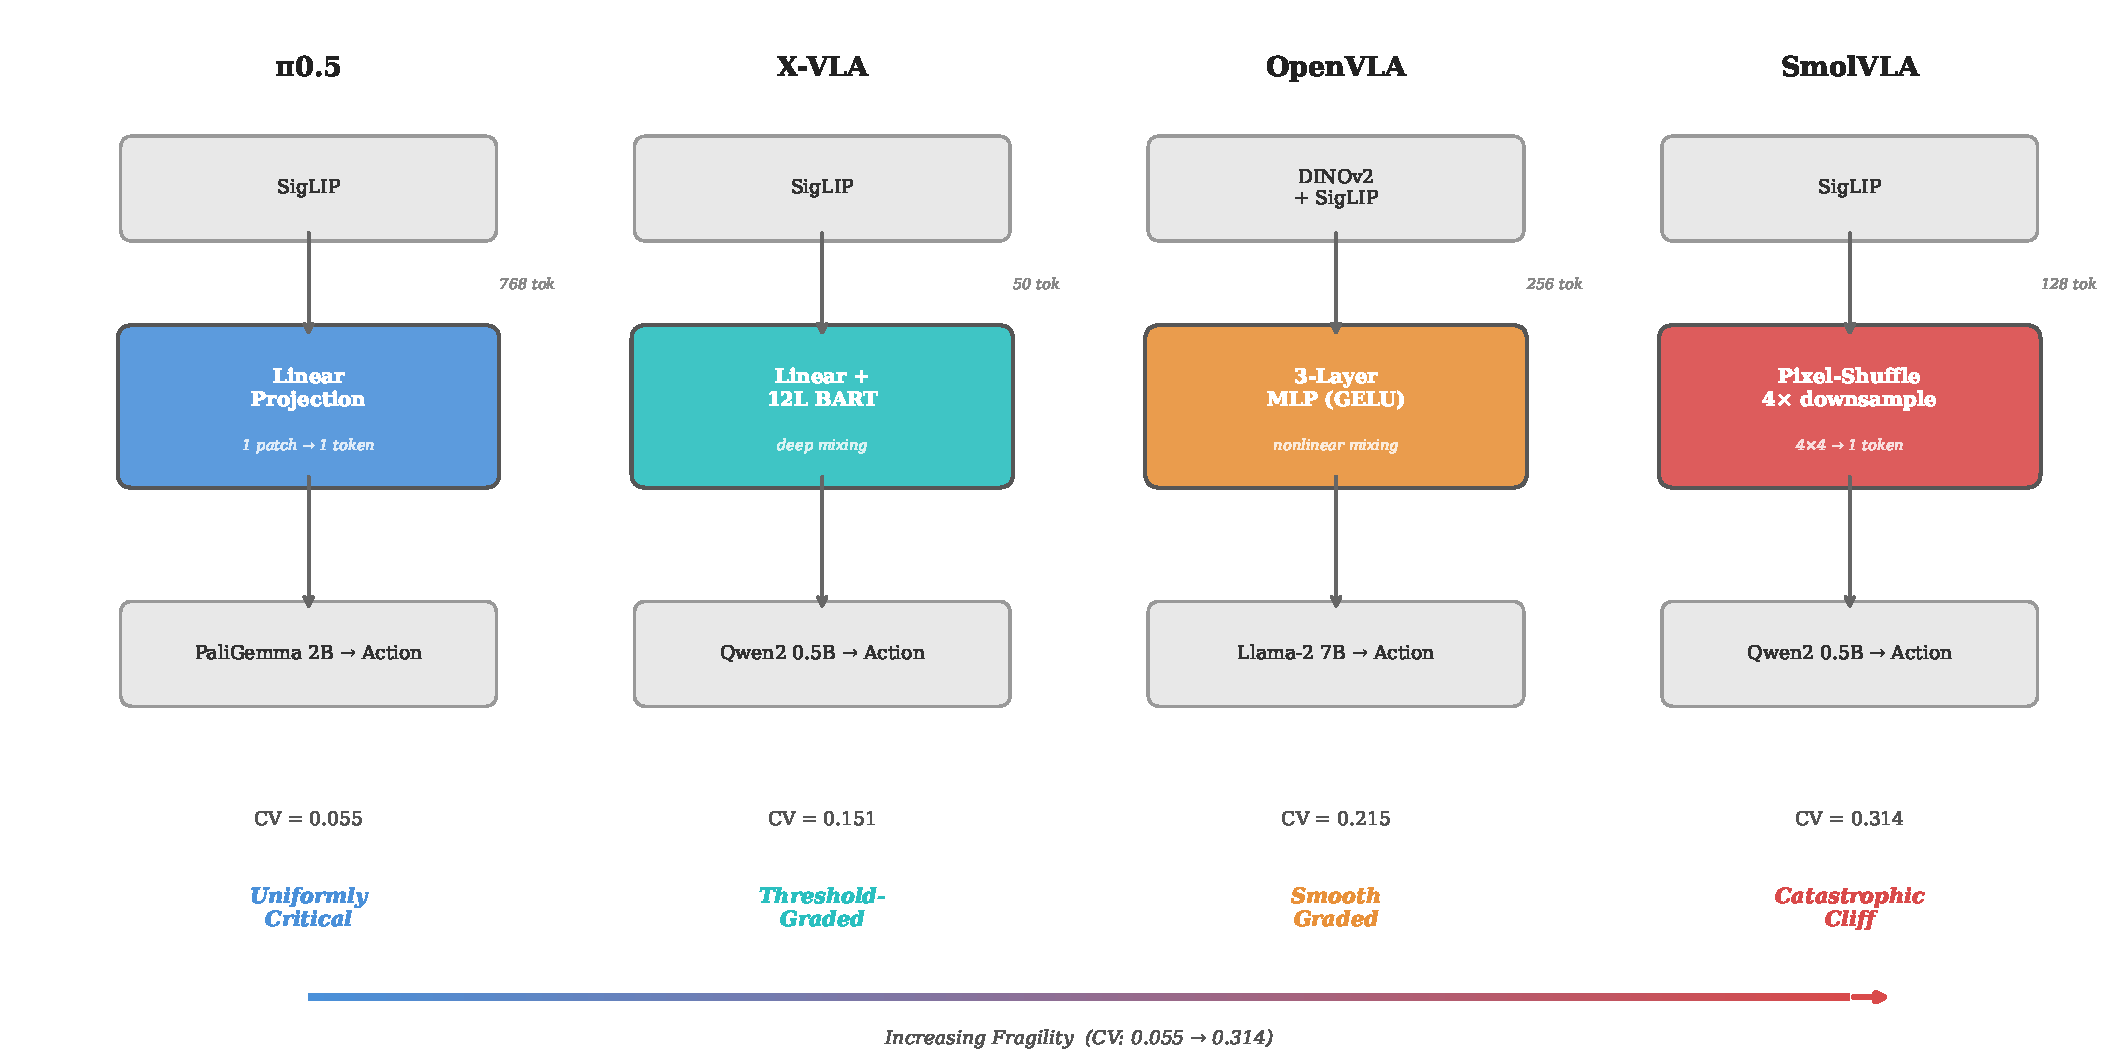
\includegraphics[width=\linewidth]{figures/paper/fig_architecture.pdf}
\caption{SmolVLA architecture and token flow. Each camera image is encoded by SigLIP into 128 spatial patch tokens. An MLP connector projects these tokens into the LLM embedding space. The Qwen2-0.5B backbone processes the concatenated vision and language tokens, and a flow matching head generates continuous 7-DoF actions.}
\label{fig:architecture}
\end{figure}

\paragraph{Vision encoder.}
SmolVLA uses the Sigmoid Loss for Language-Image Pre-training (SigLIP) encoder~\cite{zhai2023siglip} to process visual input.
SigLIP divides each camera image into non-overlapping spatial patches and encodes them independently, producing 128 tokens per image.
Two properties of this encoding are relevant to our analysis.
First, SigLIP does not include a \texttt{[CLS]} aggregation token; there is no single summary representation that pools information across patches.
Second, because patches are non-overlapping, each token encodes a unique spatial region of the input image, and no two tokens carry redundant information.
These design choices mean that the 128-token output is a spatially complete, non-redundant representation of the scene.

\paragraph{Dual-camera input.}
SmolVLA receives images from two cameras: a wrist-mounted camera (cam1) and an overhead camera (cam2).
Each camera image produces 128 vision tokens through the SigLIP encoder, yielding 256 vision tokens total that enter the language model.
The two viewpoints are complementary: the wrist camera captures fine-grained end-effector interactions, while the overhead camera provides a global spatial layout of objects on the workspace.

\paragraph{MLP connector.}
A multi-layer perceptron (MLP) projects each SigLIP output token from the vision encoder embedding space into the Qwen2-0.5B embedding space.
This connector applies a learned linear transformation per token without cross-token interaction, preserving the one-to-one correspondence between spatial patches and tokens.
The intervention point for token reduction in our experiments sits immediately after this connector: pruning, masking, or merging operations are applied to the projected vision tokens before they enter the language model.

\paragraph{LLM backbone.}
The Qwen2-0.5B language model~\cite{yang2024qwen2} serves as the central reasoning module.
It receives a concatenated input sequence of 256 projected vision tokens and the tokenized language instruction.
Self-attention across this full sequence allows the model to ground language in visual context and to integrate information across both camera views.
The backbone must reconcile spatial relationships between the robot gripper, target objects, and obstacles using only the vision tokens, since no other spatial input is provided.

\paragraph{Flow matching action head.}
SmolVLA generates actions through conditional flow matching~\cite{lipman2023flow} rather than autoregressive token prediction.
The action head maps the LLM's output representation to a continuous 7-DoF action vector: three position coordinates, three rotation angles, and one gripper open/close value.
Flow matching learns a vector field that transports a noise distribution to the target action distribution, conditioned on the LLM output.
This formulation produces smooth, continuous actions suited to precise manipulation, but it also means that the action output depends holistically on the LLM's internal representation.
Any corruption of the vision token input propagates through the full LLM computation into the predicted action.

The overall inference pipeline proceeds as: image $\rightarrow$ SigLIP patches $\rightarrow$ 128 tokens per camera $\rightarrow$ MLP projection $\rightarrow$ concatenation with language tokens $\rightarrow$ Qwen2-0.5B forward pass $\rightarrow$ flow matching action prediction.
This architecture shares its high-level structure with larger VLA systems such as OpenVLA~\cite{kim2024openvla} and $\pi_0$~\cite{black2024pi0}, making SmolVLA a representative testbed for studying vision token efficiency in VLA policies.

\subsection{LIBERO Benchmark}
\label{sec:libero_bench}

We evaluate on the LIBERO benchmark~\cite{liu2023libero}, a suite of language-conditioned tabletop manipulation tasks in simulation.
LIBERO provides standardized task definitions, initial state distributions, and evaluation protocols for reproducible comparison of manipulation policies.
We use three of its four suites, each testing a distinct aspect of policy competence.
LIBERO-Object presents ten tasks focused on object manipulation; the policy must identify and interact with specific objects from visually similar alternatives.
LIBERO-Spatial presents ten tasks focused on spatial reasoning, where the policy must place objects correctly or navigate relative to reference locations.
LIBERO-Goal presents ten tasks with varied goal conditions applied to a shared environment layout; these tasks test whether the policy can condition its behavior on the language instruction.

Each suite contains 10 tasks, and we run 50 evaluation episodes per task, yielding 500 episodes per suite per experimental condition.
The evaluation metric is closed-loop Success Rate (SR): a binary indicator per episode that equals 1 only if the robot completes the full task within the time limit.
SR is measured through closed-loop execution, where the policy observes the current state, predicts an action, the simulator advances, and the policy re-observes the updated state at every timestep.
This closed-loop evaluation is critical because errors at any single step can cascade through subsequent observations and actions.
A policy that produces even one qualitatively wrong action (for example, opening the gripper when it should close) will likely fail the entire episode.

The three LIBERO suites span a range of baseline difficulty levels: SmolVLA achieves 44.8\% SR on Object, 51.8\% on Spatial, and 63.0\% on Goal in bypass mode (full vision tokens, no pruning).
These baseline numbers are not state-of-the-art; SmolVLA is a compact model designed for efficiency research.
The relevant comparison is not the absolute success rate but the change under token reduction: any viable pruning strategy must approximately preserve these baselines rather than collapse to 0\%.
